%-------------------
% CHAPTER 6: Design
%-------------------

\chapter{Design}

\label{chapter06}

With all the specification of the data the \thesis\ will work with, a good architecture for the system is needed. The whole software project is split in four different parts: Available Flights Pipeline, User Searches Pipeline, Comparison Service and Web UI.
\\\\
In this chapter all four architectures for the four different parts will be defined and analyzed. All alternatives will also be defined and explain why it is not in the final architecture.
\\\\
Even so, first it is good to understand the general architecture of the whole \thesis.

%-----------------
%   SECTION 6.1
%-----------------

\section{Architecture}

The \thesis\ is split in very notable three layers: Data collection and processing, Comparison Server and Web UI. Two of this layer, server and user interface, suit exactly two of the four remarkable in the whole system, the Comparison Service and Web UI. Named the same to avoid confusion.
\\\\
An important characteristic of the \thesis\ is that the only way to feed the database is from the data collection and processing layer. This is different of most of projects and examples I have worked before in the University.
\\\\
The most common architecture used is a three layers (data layer, domain layer and presentation layer) where in the presentation layer the user could usually put data into the data layer. The \thesis\ work very different: The user interface (that is the presentation layer) does not put or modifies any data from the database. It only reads. The only way the database can be filled with valid data is from the \textit{data collection and processing layer}.

\begin{figure}[H]
\centering
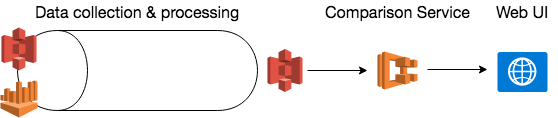
\includegraphics[scale=0.7]{diagrams/architecture01.png}
\caption{General view of the \thesis\ architecture.}
\end{figure}

% SUB SECTION 6.1.1

\subsection{Data collection and processing} \label{data_layer}

This layer is composed by two components, one for each data processing: Available Flights Pipeline and User Searches Pipeline. The purpose of this layer is to collect all data necessary to do the comparison and filter and group according the final data model needed.
\\\\
Both components in the this layer uses very similar technologies and are written in Scala\cite{scala}. The data is read from different sources that already exist in \company\ and have a well defined design (\nameref{data_tribe} and \squad's pipeline) and services (\nameref{athena} and \nameref{s3}, S3). The whole data processing or data pipeline ran in Apache Spark, in an EMR cluster. In the end of the process both pipelines write into the same Storage service.

\begin{figure}[H]
\centering

\includegraphics[scale=0.7]{diagrams/architecture-data.png}
\caption{General view of the data collection and processing layer's architecture.}
\end{figure}

\subsubsection{Amazon Athena} \label{athena}

\begin{figure}[H]

\includegraphics[scale=0.1]{resources/athena-logo.png}
\end{figure}

Amazon Athena\cite{athena}, is an Amazon Web Service that lets query data stored in \nameref{s3} (S3) using standard SQL\cite{sql}. It have no server running, so it have no infrastructure to manage.
\\\\
To access the data, Athena simply points to an S3 bucket with a defined schema and it lets you query its data with SQL queries. The cost of the service is based on the queries you run.
\\\\
\nameref{data_tribe} is responsible of creating schemas for Athena to read S3 buckets. They have a huge bucket called \texttt{grappler\_master\_archive} that contains all the user searches. Athena becomes the easiest way to access user searches data.

\subsubsection{Amazon Simple Storage Service} \label{s3}

\begin{figure}[H]

\includegraphics[scale=0.1]{resources/s3-logo.png}
\end{figure}

Amazon Simple Storage Service\cite{s3}, also known as \textit{S3}, stores data as objects within resources called buckets. It allows store unlimited objects in a bucket, also write, read and delete those objects. The maximum size of these objects is 5 terabytes. The access to buckets can be controlled.
\\
In \company, most of the results of \nameref{data_pipeline}s are stored as a single or multiple files in S3, then those are processed by \nameref{lambda} functions or other services. \squad\ stores timetables as a JSON\cite{json} file in its S3 bucket. Data tribe has also a bucket for user searches (and much more) data, but, as explained before, it provides access from \nameref{athena}.

\subsubsection{Apache Spark\textsuperscript{TM}} \label{apache_spark}

\begin{figure}[H]

\includegraphics[scale=0.1]{resources/apache-spark_logo.png}
\end{figure}

Apache Spark\textsuperscript{TM} is a unified analytics engine for large-scale data processing. It was created and it is currently maintained by the Apache Software Foundation\cite{apache_software_foundation}.
\\\\
Is one of the most popular fast and general-purpose cluster computing systems. It can run in a lot of different environments, Apache\textsuperscript{TM} Hadoop\textregistered\cite{hadoop}, Kubernetes\cite{k8s}, \nameref{emr} and much more. Spark provides four APIs: Java, Scala, Python, R and SQL. Over 80 high-level operators can help building parallel processes and can be called from most of its APIs. Both data pipelines are written using the Scala API.
\\\\
Apache Spark\textsuperscript{TM}'s architecture is based in \textit{Resilient Distributed Datasets}, RDD, a read-only multiset distributed in multiple machines. Those machines are based in the MapReduce paradigm, a programming model for big data dumps processing. Since the data is distributed, this process runs in parallel.
\\\\
To an RDD, you can apply two kind of operations: transformations and actions:
\\\\
A \textbf{Spark Transformation} is a functions that creates a new RDD form the existing one. Transformations are lazy operations and only are executed when an action is called. When calling a transformation, a link is created between two RDDs, this happens successively until the action is executed. Then, all transformations are applied until the action. These links between transformations creates a directed acyclic graph.

\begin{figure}[H]
\centering
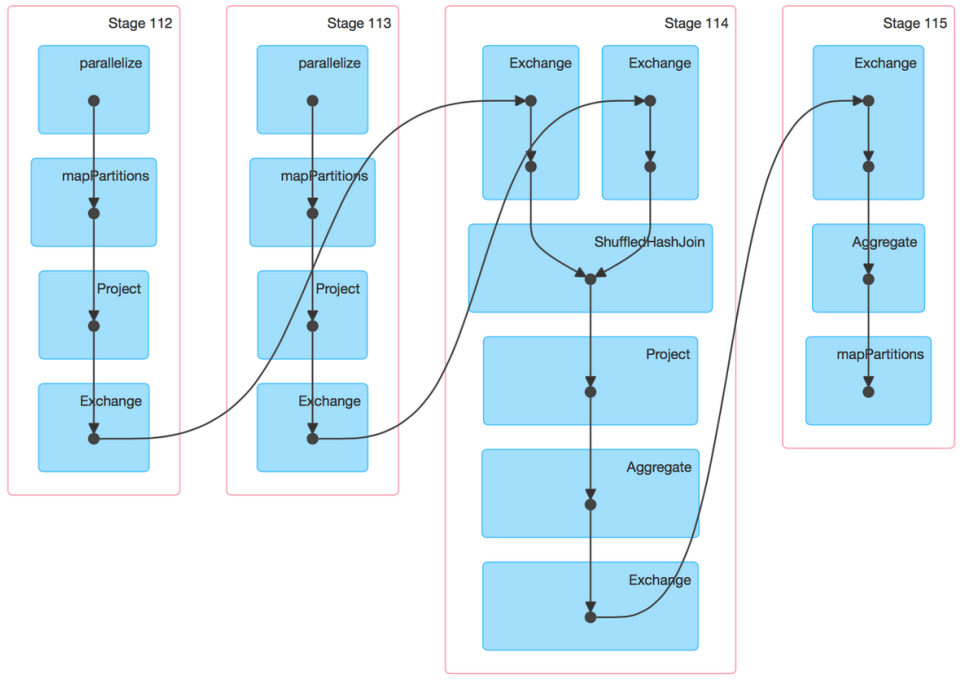
\includegraphics[scale=0.3]{resources/dag.png}
\caption{Example of a Directed Acyclic Graph (DAG).}
\end{figure}

Most common transformations used in the project are:

\begin{displayquote}
\texttt{def map[R](f: Function[T, R]): RDD[R]}
\\
Return a new RDD by applying a function to all elements of this RDD.
\\\\
\texttt{def flatMap[U](f: FlatMapFunction[T, U]): RDD[U]}
\\
Return a new RDD by first applying a function to all elements of this RDD, and then flattening the results.
\\\\
\texttt{def filter(f: Function[T, Boolean]): RDD[T]}
\\
Return a new RDD containing only the elements that satisfy a predicate.
\\\\
\texttt{def groupBy[U](f: Function[T, U]): PairRDD[U, Iterable[T]]}
\\
Return an RDD of grouped elements. Each group consists of a key and a sequence of elements mapping to that key.
\end{displayquote}

A \textbf{Spark Action} are RDD operations that do not return an RDD-like value. Actions are executed when called, first running all transformation in the directed acyclic graph of transformations.
\\\\
Most common actions used in pipelines are:

\begin{displayquote}
\texttt{def count(): Long}
\\
Return the number of elements in the RDD.
\\\\
\texttt{def fold(zeroValue: T)(f: Function2[T, T, T]): T}
\\
Aggregate the elements of each partition, and then the results for all the partitions, using a given associative function and a neutral "zero value".
\\\\
\texttt{def foreach(f: VoidFunction[T]): Unit}
\\
Applies a function f for all elements of this RDD.
\end{displayquote}

\subsubsection{Amazon Data Pipeline} \label{data_pipeline}

\begin{figure}[H]

\includegraphics[scale=0.1]{resources/data_pipeline-logo.png}
\end{figure}

Amazon Data Pipeline\cite{data_pipeline} service helps running processes reliably and move data between Amazon Web Services Storage services. In the \thesis\ it is used to move data From \nameref{athena} or \nameref{s3} to \nameref{emr} and from \nameref{emr} back to \nameref{s3}.
\\\\
If, for any reason, the pipeline fails, this service retries the execution, if the execution fails constantly, the data pipeline stops and sends a failure notification to the owner.
\\\\
Data Pipelines can also be scheduled to run every hour, every two hours, every day, week, etc. Both pipelines are scheduled to run once a day every day. In every executions, first builds the environment (\nameref{emr} and \nameref{apache_spark}) and then runs the JAR\cite{jar} file generated from available flights pipeline and user searches pipeline. To avoid unnecessary dependencies, there are two \nameref{data_pipeline}s, one for the flights and another for the user searches.

\subsubsection{Amazon Elastic MapReduce} \label{emr}

\begin{figure}[H]

\includegraphics[scale=0.1]{resources/emr-logo.png}
\end{figure}

Amazon Elastic MapReduce\cite{emr} (EMR) provides a Hadoop\cite{hadoop} framework that makes easy, fast, and cost-effective to process vast amounts of data. As explained before, \nameref{apache_spark} runs in Hadoop. These clusters are prefect for running big data applications and pipelines.
\\\\
EMRs use master/slave communication model. This, applied to \nameref{apache_spark}, means that one cluster divides the data and does the partition of the RDDs while the rest of the instances, the slaves, execute the actions and transformations.
\\\\
The EMR configuration for each pipeline will be:

\begin{table}[H]
\centering
\begin{tabular}{|>{\raggedright\arraybackslash}p{5cm}|>{\raggedright\arraybackslash}p{5cm}|>{\raggedright\arraybackslash}p{3cm}|}
\hline
\textbf{Field}                        & \textbf{Description}                 & \textbf{Value}      \\ \hline
\textbf{Release}                      & EMR version                          & \texttt{emr-5.12.0} \\ \hline
\textbf{Cluster master instance type} & Instance type of the master cluster  & \texttt{m3.xlarge}  \\ \hline
\textbf{Cluster core instance type}   & Instance type of the slaves clusters & \texttt{m3.xlarge}  \\ \hline
\textbf{Cluster size}                 & Number of slaves clusters            & 6                   \\ \hline
\textbf{Timeout}                      & Insurance to not run forever         & 5 hours             \\ \hline
\end{tabular}
\caption{EMR configuration}
\end{table}

EMR 5.12.x was the latest version when the project started. Newer versions does not have any relevant upgrade.
\\\\
\texttt{m3.xlarge} has the following hardware specs:

\begin{table}[H]
\centering
\begin{tabular}{|>{\raggedright\arraybackslash}p{3.5cm}|>{\raggedright\arraybackslash}p{2cm}|>{\raggedright\arraybackslash}p{1.5cm}|>{\raggedright\arraybackslash}p{1.5cm}|>{\raggedright\arraybackslash}p{3.5cm}|}
\hline
\textbf{Name}                  & \textbf{API Name}  & \textbf{Memory} & \textbf{vCPUs} & \textbf{Instance Storage}    \\ \hline
M3 General Purpose Extra Large & \texttt{m3.xlarge} & 15.0 GiB        & 4              & 80 GiB (\(2 \times 40\) GiB) \\ \hline
\end{tabular}
\caption{\texttt{m3.xlarge} specs}
\end{table}

% SUB SECTION 6.1.2

\subsection{Service} \label{service}

The service is the middle layer of the \thesis. Simple Python\cite{python} Reads data written by the components in the \nameref{data_layer} layer and serves the data through an \nameref{ecs}.
% using Boto3\footnote{Boto\cite{boto3} is the Amazon Web Services (AWS) SDK for Python} 
\\\\
A \nameref{docker} container is created and managed by \nameref{ecs}. In this container a Python\cite{python} service is deployed.
% with AIOHTTP\footnote{AIOHTTP\cite{aiohttp} is an Asynchronous HTTP Client/Server library for Python. Perfect for HTTP Servers.} 

% \begin{figure}[H]
% \centering
% \includegraphics[scale=0.7]{diagrams/architecture-service.png}
% \caption{General view of the web service layer's architecture}
% \end{figure}

\subsubsection{Amazon Elastic Container Service} \label{ecs}

\begin{figure}[H]

\includegraphics[scale=0.1]{resources/ecs-logo.png}
\end{figure}

Amazon Elastic Container Service, also known as ECS\cite{ecs}, is a container management service that supports Docker\nameref{docker}. It ease the container orchestration with a simple API.

\subsubsection{Docker} \label{docker}

\begin{figure}[H]

\includegraphics[scale=0.1]{resources/docker-logo.png}
\end{figure}

Docker\cite{docker} tool that creates a container where you can run whichever application you want with its environment. A Docker container can be created in a lot of machines, for example in an \nameref{ecs}.

\subsection{Website}

Finally, the presentation layer gets data from the \nameref{service} and displays. The architecture of this layer is very simple, the website does an HTTP request to the service and gets a JSON back.
\\\\
It is also ran in a \nameref{docker} container deployed in \nameref{ecs}.
%it using \nameref{vega}. The whole website is build with the \company\ standard for \textit{frontend} \nameref{react}.

% \begin{figure}[H]
% \centering
% \includegraphics[scale=0.7]{diagrams/architecture-web.png}
% \caption{General view of the website layer's architecture}
% \end{figure}

% \subsubsection{Vega} \label{vega}

% \begin{figure}[H]
% 
\includegraphics[scale=0.88]{resources/idl-logo.png}
% \end{figure}

% \subsubsection{React.js} \label{react}

% \begin{figure}[H]
% 
\includegraphics[scale=0.1]{resources/react-logo.png}
% \end{figure}

%-----------------
%   SECTION 6.2
%-----------------

\section{Components}

Once the technology each layer will use, lets define the code architecture of each component.

\subsection{Available Flights Pipeline} \label{available-flights-pipeline}

The flight offer data pipeline reads timetables from \squad's ingest pipeline, stored in \nameref{unified-model} and group, map and filter to \nameref{flight-availablity-model}.
\\\\
\squad's Ingest Pipeline writes all the timetables in its \nameref{s3} bucket in very JSON\cite{json} alike format. \nameref{apache_spark} and the components of \squad\ that read routes from the result file line by line, each of those lines is a Unified Route. Luckily when Apache Spark reads a file i creates an RDD of String, one record per line; so when reading \squad's file, it will get an RDD of Unified Routes in JSON\cite{json} format.
\\\\
For all data processing, the pipeline is split in well-defined stages. Each stage has a name to be identified and a function \texttt{run} that executes the Spark transformations and actions needed to complete its purpose. The Available Flights Pipeline is composed by six stages grouped in two \textit{sub-pipelines}:

\subsubsection*{Routes \textit{sub-pipeline}}

This \textit{sub-pipeline} basically regroup Unified Routes data to a friendly model for the Routes Availability. It does not discards any field just in case those want to be used for future features, improvements or applications.

\begin{itemize}
    \item \textbf{Read Routes stage}: It reads the \texttt{version.txt} file from \squad's bucket, there it get the latest version of the timetables and read them, returning an Strings RDD.
    \item \textbf{JSON to Route stage}: Maps from a String RDD to a Unified Route Class using \nameref{Gson}.
    \item \textbf{Flights Flattening stage}: Flats all routes' series at date level, duplicating origins and destinations since each flight have the same route. There are three flattening, from series to series item, from series item to date sets and finally from date sets to single dates. Going from 64,000 routs to 75,000,000 flights. The amount of data increases a lot here.
    \item \textbf{Group Routes stage}: After flattening at date level, flights are grouped by date. There is a lot of shuffling\footnote{Sharing data between different nodes or machines} which makes it a slow process.
\end{itemize}

Apart from these four stages, it has other to parse grouped routes by date objects to JSON\cite{json} and another to write it to \nameref{s3}, but since in the end those are not necessary, these two stages are disabled.

\subsubsection*{Summary \textit{sub-pipeline}}


\begin{itemize}
    \item \textbf{Map Summary stage}: Discards lots of fields from the model resulting from the routes \textit{sub-pipeline} and maps the data to the final records that will be written in the database.
    \item \textbf{Write Records stage}: Writes into \nameref{s3} using \nameref{scala_aws}.
\end{itemize}

\begin{figure}[H]
\centering
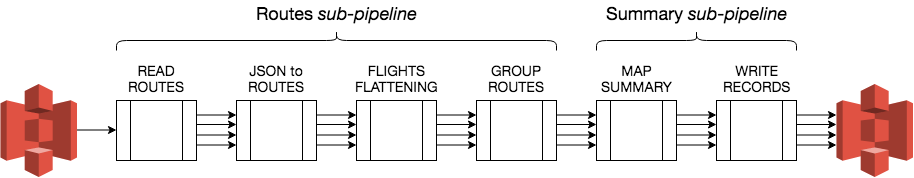
\includegraphics[scale=0.45]{diagrams/available-flights-pipeline-architecture.png}
\caption{Available flights pipeline architecture and data flow diagram}
\end{figure}

To end up doing applying this architecture, there have been a lot of alternatives during all the development of the Available Flights Pipeline.

\subsubsection{Amazon Relational Database Service} \label{rds}

\begin{figure}[H]

\includegraphics[scale=0.1]{resources/rds-logo.png}
\end{figure}

In the beginning, the idea was to write all data to Amazon RDS, Relational Database Service\cite{rds}. This service offers a relational database in the cloud that can be accessed very fast. But there are two important reasons thy this option has been discarded:

\begin{itemize}
    \item \textbf{Cost}: It is very expensive to have an RDS active all the time. Some squads in \company\ use \nameref{rds} but only active some time a week for very specific purposes.
    \item \textbf{Knowledge}: I know about some squads that used that in some occasion, but not based in Barcelona. Reading some documentations and examples, it looked very difficult to set up and use, there were alternatives 
\end{itemize}

\subsubsection{Amazon DynamoDB} \label{dynamodb}

\begin{figure}[H]

\includegraphics[scale=0.2]{resources/dynamodb-logo.png}
\end{figure}

Another idea about the database where the pipeline could write was Amazon RDS, Relational Database Service\cite{dynamodb}. This service offers a non-relational database in the cloud that can be accessed very fast. But there was one important reasons thy this alternative was discarded:

\begin{itemize}
    \item \textbf{Cost}: It is very expensive to have an DynamoDB, even more expensive than \nameref{rds}.
\end{itemize}

\subsubsection{S3 and dates at month level} \label{month_version}

The main problem of these pipeline that happens in the \nameref{user-searches-pipeline} as well, is that \textbf{versions are written every day} and does not delete anything to satisfy functional requirement of Historical data (\#8)
\\\\
\squad\ provides flights for one year ahead and every day the data is uploaded in a new file to S3, the \nameref{available-flights-pipeline} reads this file and gets all flights for all days in the next year and writes them to the Database. It would be very easy for the service then read with an SQL table like:

\begin{table}[H]
\centering
\begin{tabular}{|>{\raggedright\arraybackslash}p{2.5cm}|>{\raggedright\arraybackslash}p{2.5cm}|>{\raggedright\arraybackslash}p{3cm}|>{\raggedright\arraybackslash}p{3cm}|>{\raggedright\arraybackslash}p{2.5cm}|>{\raggedright\arraybackslash}p{2.5cm}|>{\raggedright\arraybackslash}p{1cm}|}
\hline
\texttt{origin}       & \texttt{destination}   & \texttt{version\_date}       & \texttt{flight\_date}        & \texttt{count}       \\ \hline
BCN                   & LGW                    & 2018-06-13                   & 2018-08-20                   & 14                   \\ \hline
BCN                   & LGW                    & 2018-06-13                   & 2018-08-21                   & 12                   \\ \hline
BCN                   & MAD                    & 2018-06-13                   & 2018-08-20                   & 34                   \\ \hline
\cellcolor{blue!5}BCN & \cellcolor{blue!5}EDI  & \cellcolor{blue!5}2018-06-13 & \cellcolor{blue!5}2018-08-12 & \cellcolor{blue!5}20 \\ \hline
\cellcolor{blue!5}BCN & \cellcolor{blue!5}EDI  & \cellcolor{blue!5}2018-06-14 & \cellcolor{blue!5}2018-08-12 & \cellcolor{blue!5}20 \\ \hline
\cellcolor{blue!5}BCN & \cellcolor{blue!5}EDI  & \cellcolor{blue!5}2018-06-15 & \cellcolor{blue!5}2018-08-12 & \cellcolor{blue!5}30 \\ \hline
BCN                   & EDI                    & 2018-06-15                   & 2018-09-14                   & 25                   \\ \hline
...                   & ...                    & ...                          & ...                          & ...                  \\ \hline
\end{tabular}
\end{table}

So, for instance, if the user queries for the evolution of the flights available from Barcelona to Edinburgh on August 12 of 2018, the service could simple run an SQL query to the Database like \texttt{SELECT * FROM flight\_availability WHERE origin = "BCN" AND destination = "EDI" AND flight\_date = "2018-08-12"}. Then the service could map the result to the desired schema and response it back to the client.
\\\\
Looks easy and simple, but the problem is that, as explained before, \nameref{rds} is very expensive. The only storage service left that does not take much time to develop is \nameref{s3}.
\\\\
Is very fast to write to S3, the whole data dump with more than 75 million flights can be written in less than a minute to a single flight, but how about the reading from the service? Boto3\footnote{Boto\cite{boto3} is the Amazon Web Services (AWS) SDK for Python, explained in \nameref{boto3} on page \pageref{boto3}} takes more or less an eighth of a second to access the file and more or less a quarter second to read the whole file. This is fine if the service just needs to read one file, but as explained before, the pipeline writes one file every day. So, for one query, the worst case scenario is 365 (one year) files to open and read. In other words, more than 4 minutes for the service to response a query. This does not satisfy the fourth non-functional requirement of Speed and Latency.
\\\\
After analyzing the data, one solution was to only write changes, so there are no that big amount of files to read, but it was discarded because user searches change every day, not like flights, and the same problem would happen when reading from the other pipeline.
\\\\
In the end, the final solution was to write one file per record, and inside it all the data about the flights for that route in that date. That way, \nameref{boto3} could run the \texttt{list\_bucket} function, that list all objects under the given key.

\begin{verbatim}
BCN-LGW/
        2018-08-20/
                   2018-06-13-14.json
        2018-08-21/
                   2018-06-13-12.json

BCN-MAD/
        2018-08-20/
                   2018-06-13-34.json

BCN-EDI/
        2018-08-12/
                   2018-06-13-20.json
                   2018-06-13-20.json
                   2018-06-13-30.json
        2018-09-14/
                   2018-06-15-25.json
\end{verbatim}

The problem with that is that there are 75 million different records to write. It would take more than one day for the pipeline to write the whole data, very expensive because of the \nameref{emr} cluster running time and very slow. 
\\\\
After checking the user stories and the purpose of this tool, a final decision was made: Data was going to be store that way, one record per day, but the number of records will be reduced to much \textbf{grouping flights at month level} instead of at day level. The final S3 directory structure would be:

\begin{verbatim}
BCN-LGW/
        2018-08/
                2018-06-13-26.json

BCN-MAD/
        2018-08/
                2018-06-13-34.json

BCN-EDI/
        2018-08/
                2018-06-13-20.json
                2018-06-13-20.json
                2018-06-13-30.json
        2018-09/
                2018-06-15-25.json
\end{verbatim}

With this design, the service takes less than a second to get all the data and the pipeline takes one hour to write all the records.

\subsection{User Searches Pipeline} \label{user-searches-pipeline}

The user demand is obtained from \textbf{user searches} table in \nameref{athena}. Then the results of the Athena query are mapped to the same data model of the stored in S3 by the \nameref{available-flights-pipeline}.
\\\\
The first problem found in this pipeline was that the results from Athena were stored in a CSV\cite{csv} in S3 and each row had a record with a format very similar than JSON\cite{json}. Those records could not be parsed to an object using any library\footnote{Solution explained in \nameref{regex} on page \pageref{regex}}.
\\\\
Another problem found is that as more data you request, more time it gets to finish the query, and it is not a lineal progression. To solve that, the query was split in four sub-queries. From one query that requested all the user flight searches for one day to four that request all user flight searches in hour ranges 00:00-05:59, 06:00-11:59, 12:00-17:59 and 18:00-23:59. Usually the resultant files take \textbf{30 gigabytes}.
\\\\
\nameref{user-searches-pipeline} is not split in \textit{sub-pipelines}. It has four stages in total:

\begin{itemize}
    \item \textbf{Athena Reader stage}: Queries Athena for user searches. Athena writes automatically to S3 and returns the file name.
    \item \textbf{S3 Reader stage}: Gets the file name of the query result and reads it. CSV\cite{csv} to String RDD.
    \item \textbf{Search Query stage}: Gets the records from the Athena records, filters them by kind of search an other parameters, maps each record to the desired model and groups by route.
    \item \textbf{Write Records stage}: Writes into \nameref{s3} using \nameref{scala_aws}.
\end{itemize}

\begin{figure}[H]
\centering
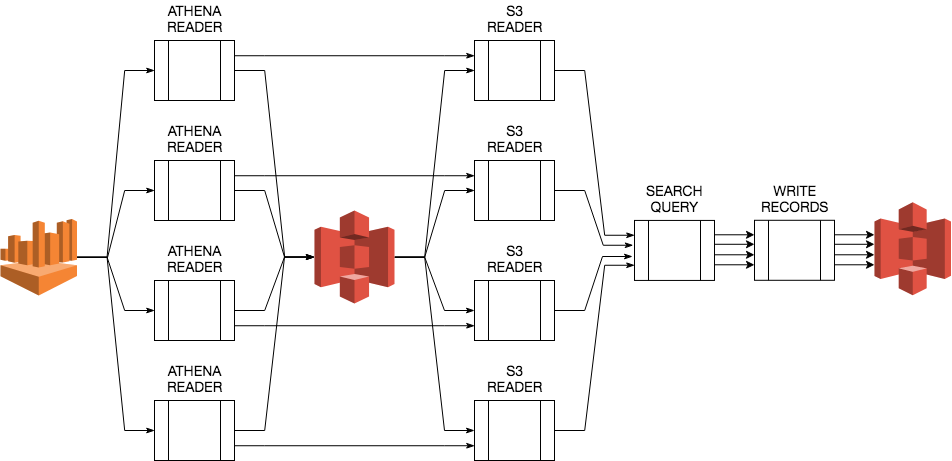
\includegraphics[scale=0.45]{diagrams/user-searches-pipeline-architecture.png}
\caption{User searches pipeline architecture and data flow diagram.}
\end{figure}

\subsection{Comparison Service}

Once all the data is processed every day and stored into \nameref{s3}, it has to be served in an HTTP\cite{http} API.
\\\\
The Comparison Servie's API provides two endpoints, one for the comparison and another one for a single source (flights or searches) request\footnote{The \textit{endpoint} tag can be \texttt{sandbox} or \texttt{prod}. Learn more about those environments in section \nameref{environments} on page \pageref{environments}.}. The main class, API Handler, execute a function when the endpoint is queried and uses an AWS Adapter that is directly connected to \nameref{boto3}. The API Handler returns a set of records in JSON format.

\begin{figure}[H]
\centering
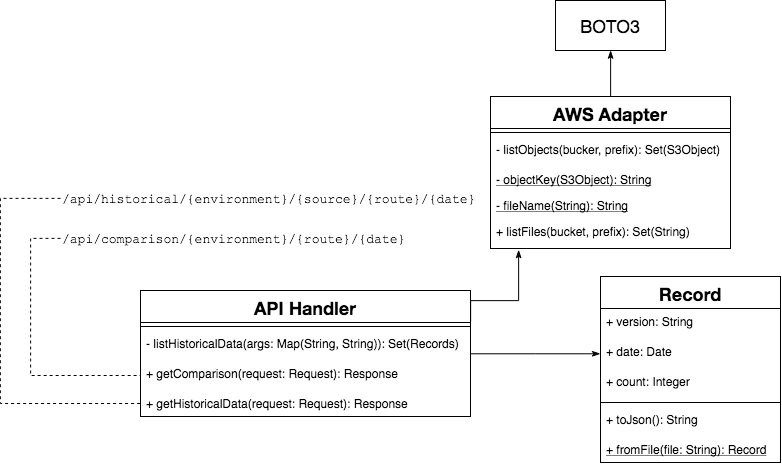
\includegraphics[scale=0.5]{diagrams/server-architecture.png}
\caption{Comparison service class diagram.}
\end{figure}

\textbf{\texttt{/api/comparison/{environment}/{route}/{date}}}
\\\\
GET two sets of data for a given route and date: All existent versions values for available flights and user searches.
\\\\
\textbf{\texttt{/api/historical/{environment}/{source}/{route}/{date}}}
\\\\
GET one sets of data for a given route and date and source\footnote{The two available source the Service have are: Available Flights and User Searches}: All existent versions.

The first idea for the comparison service, was using an AWS Lambda Function and exposing it through AWS API Gateway. But it ended up in \nameref{ecs} with a \company\ gateway.

\subsubsection{Amazon Lambda} \label{lambda}

\begin{figure}[H]

\includegraphics[scale=0.1]{resources/lambda-logo.png}
\end{figure}

Is one of the most uses service used bu Amazon Web Service. It is a \textit{serverless} system that lets you run code easily.

\begin{displayquote}
\textit{Run code without thinking about servers. Pay only for the compute time you consume.}
\end{displayquote}

Lambda functions can be executed from an S3 event (run a lambda when a file under a given prefix is putted in a bucket) or an API Gateway, it get an event and a context input, runs Python\cite{python} or Node.js\cite{nodejs} code and returns (or not) some value. By default Lambdas have a three minutes timeout, which is not a problem. Also, Lambdas \textbf{scale automatically}.
\\\\
This service looked very promising but was not used because of API Gateways.

\subsubsection{Amazon API Gateway}

\begin{figure}[H]

\includegraphics[scale=0.2]{resources/api-logo.png}
\end{figure}

Simple service that provides a front door for whatever other Amazon's service.
\\\\
\company\ reached the limit of API Gateways. Using a Lambda I would have open an special request in the company to get a new API Gateway, this request would have been provably reject because API Gateways are reserved for very specific uses. That is why \nameref{lambda} and API Gateway was not used for the service.

\subsection{Web UI}

Finally, in the front end of the application, the Web UI. A simple website with only one page, based in the Composite Pattern becomes a responsive application with a high code scalability and maintainability.

\begin{figure}[H]
\centering
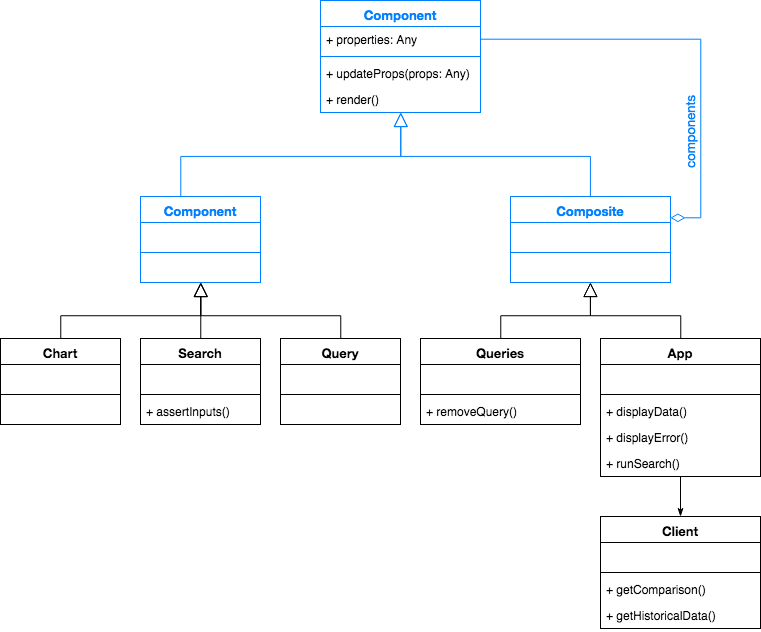
\includegraphics[scale=0.5]{diagrams/web-ui-architecture.png}
\caption{Web UI class architecture. In blue we can appreciate the Composite Pattern base classes and relations.}
\end{figure}

%-----------------
%   SECTION 6.2
%-----------------


